\documentclass{article}

\usepackage{graphicx}
\usepackage{caption}
\usepackage[a4paper,landscape,margin=1in]{geometry}
\usepackage[capbesideposition={top},facing=yes,capbesidesep=quad]{floatrow}

\begin{document}

\begin{figure}[!ht]
  \fcapside
  {
    \captionsetup{labelformat=empty}
    \caption{Frame 1:}
  }
  {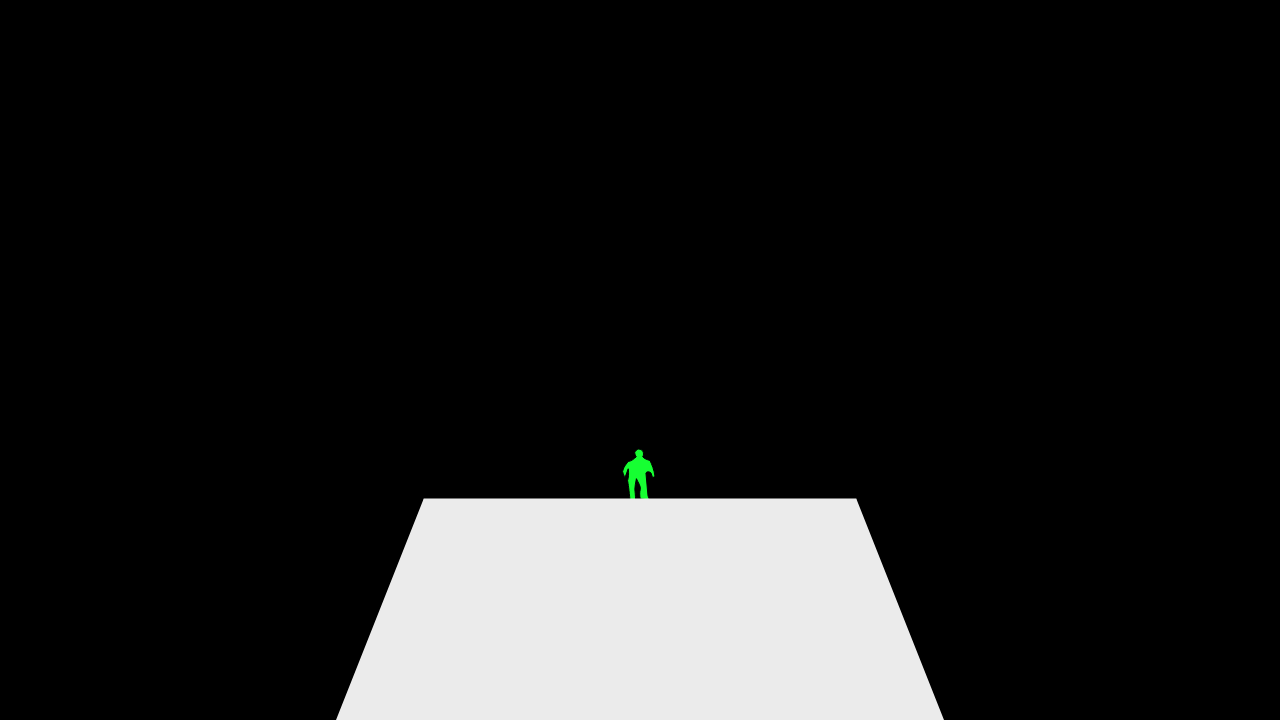
\includegraphics[width=0.45\textwidth]{Frame1.png}}
\end{figure}

\begin{figure}[!ht]
  \fcapside
  {
    \captionsetup{labelformat=empty}
    \caption{Frame 2:}
  }
  {
\includegraphics[width=0.45\textwidth]{Frame2.png}}
\end{figure}

\pagebreak

\begin{figure}[!ht]
  \fcapside
  {
    \captionsetup{labelformat=empty}
    \caption{Frame 3:}
  }
  {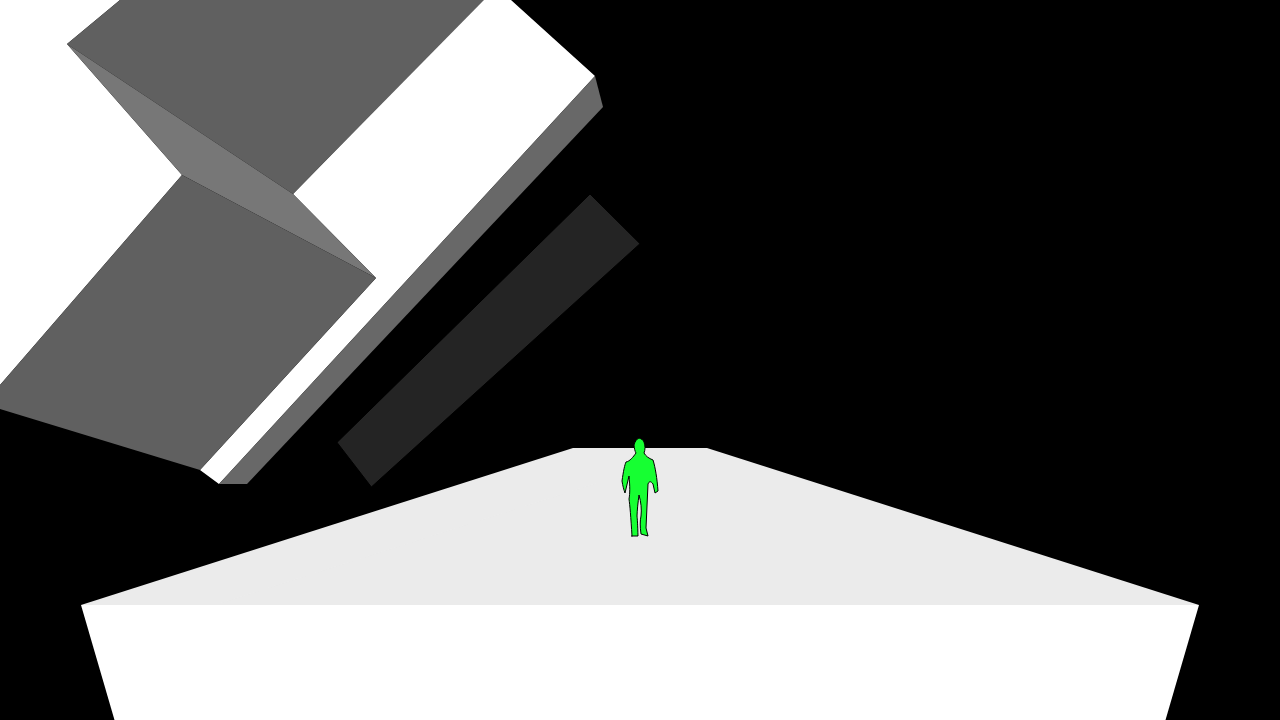
\includegraphics[width=0.45\textwidth]{Frame3.png}}
\end{figure}

\begin{figure}[!ht]
  \fcapside
  {
    \captionsetup{labelformat=empty}
    \caption{Frame 4:}
  }
  {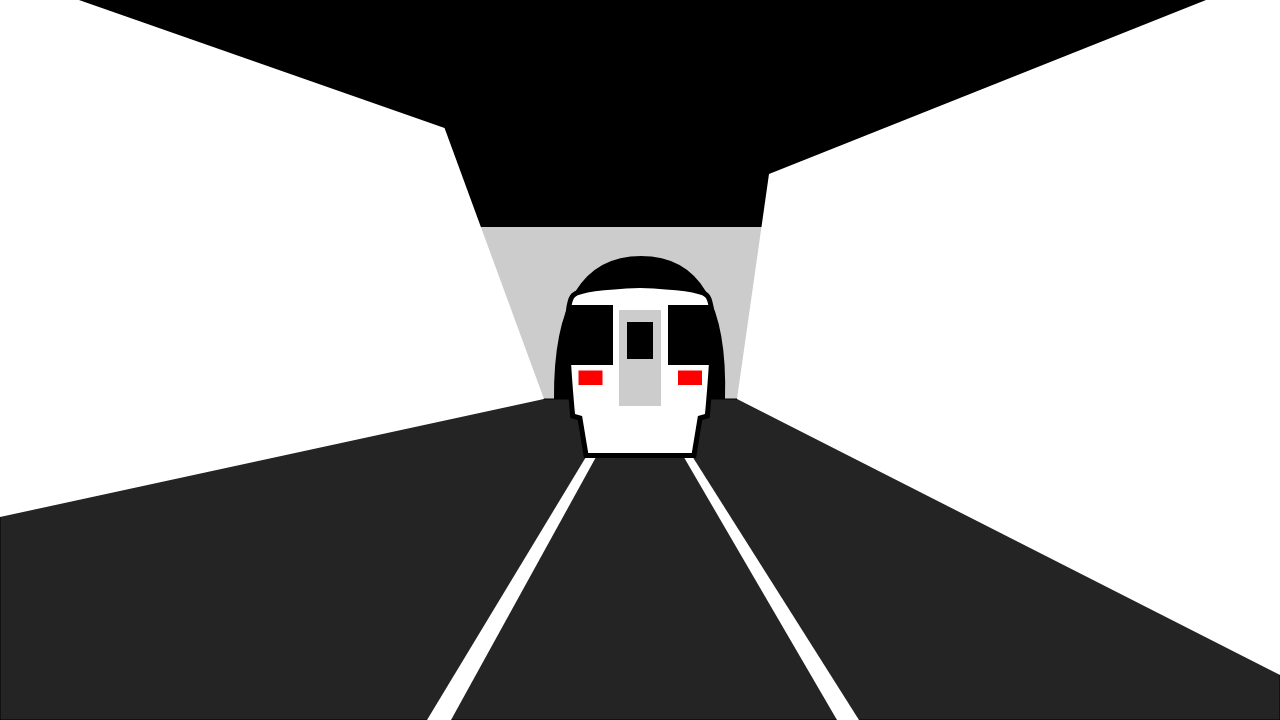
\includegraphics[width=0.45\textwidth]{Frame4.png}}
\end{figure}

\pagebreak

\begin{figure}[!ht]
  \fcapside
  {
    \captionsetup{labelformat=empty}
    \caption{Frame 5:}
  }
  {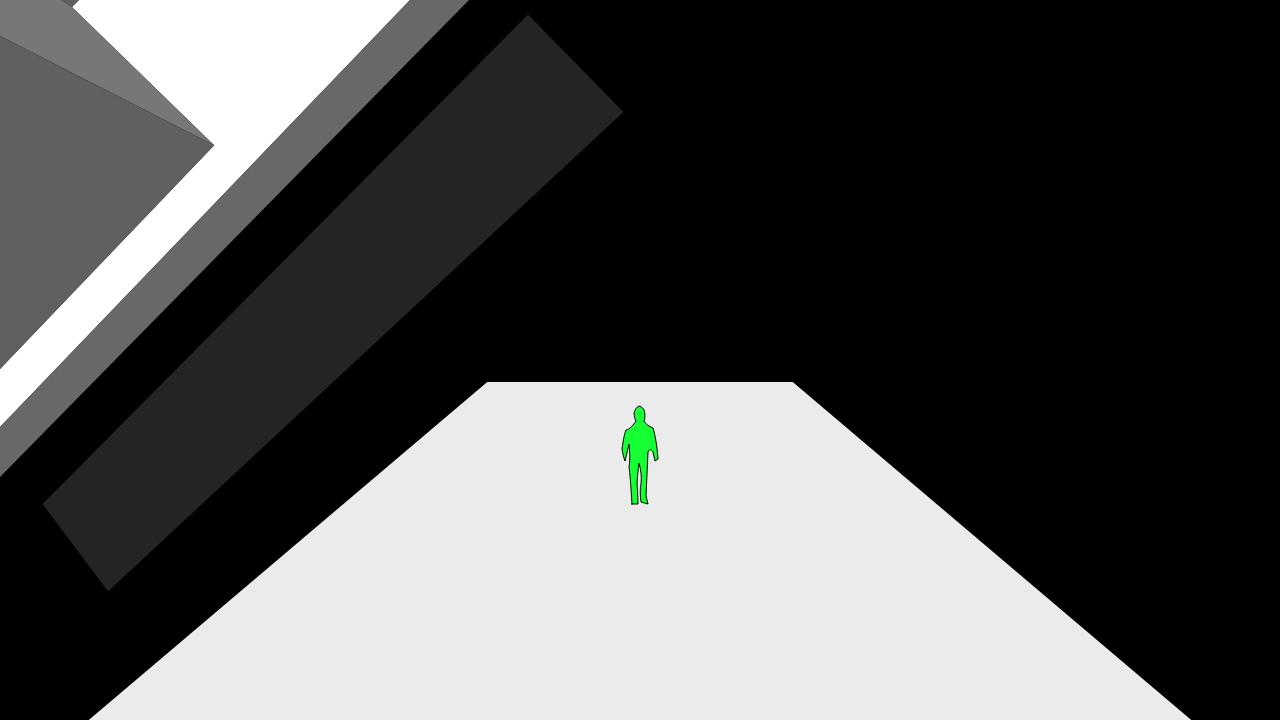
\includegraphics[width=0.45\textwidth]{Frame5.png}}
\end{figure}

\begin{figure}[!ht]
  \fcapside
  {
    \captionsetup{labelformat=empty}
    \caption{Frame 6:}
  }
  {
\includegraphics[width=0.45\textwidth]{Frame6.png}}
\end{figure}

\pagebreak

\begin{figure}[!ht]
  \fcapside
  {
    \captionsetup{labelformat=empty}
    \caption{Frame 7:}
  }
  {
\includegraphics[width=0.45\textwidth]{Frame7.png}}
\end{figure}

\end{document}
